\section{Matrix multiplication}

Multiplying matrices of a large size is often part of heavy scientific calculations and therefore an important building block in every mathematics library. Unfortunately, with an increasing size of the matrices the computation of the product becomes desperately slow due to an asymptotic runtime complexity of $\mathcal{O}(n^3)$ for a naive attempt. Therefore, several improvements have been tried to speed up the calculation like Strassen's algorithm achieving a runtime complexity of $\mathcal{O}(n^{\log_2 7}) = \mathcal{O}(n^{2.807})$ \ref{} which is faster than the naive version but still does not compute results within a satisfying time.
Nonetheless, modern computing systems can take advantage of one important aspect of the matrix multiplication which is it's embarrassing parallel nature. Each element of the output matrix can be computed completely independent. This potential may not only be used by today's CPU's vector extensions like SSE \footnote{Streaming SIMD Extensions, a vector instruction set extension by Intel supporting 128 bit wide registers to process 4 single precision floats in parallel.} or AVX \footnote{Advanced Vector Extensions, Intel's latest vector instruction set extension featuring 256 bit wide registers to process 8 single precision floats in parallel.}. Especially a GPU can make excellent use of the large number of independent pieces of work to perfectly utilize its hundreds or thousands of cores.

\begin{figure}
\centering
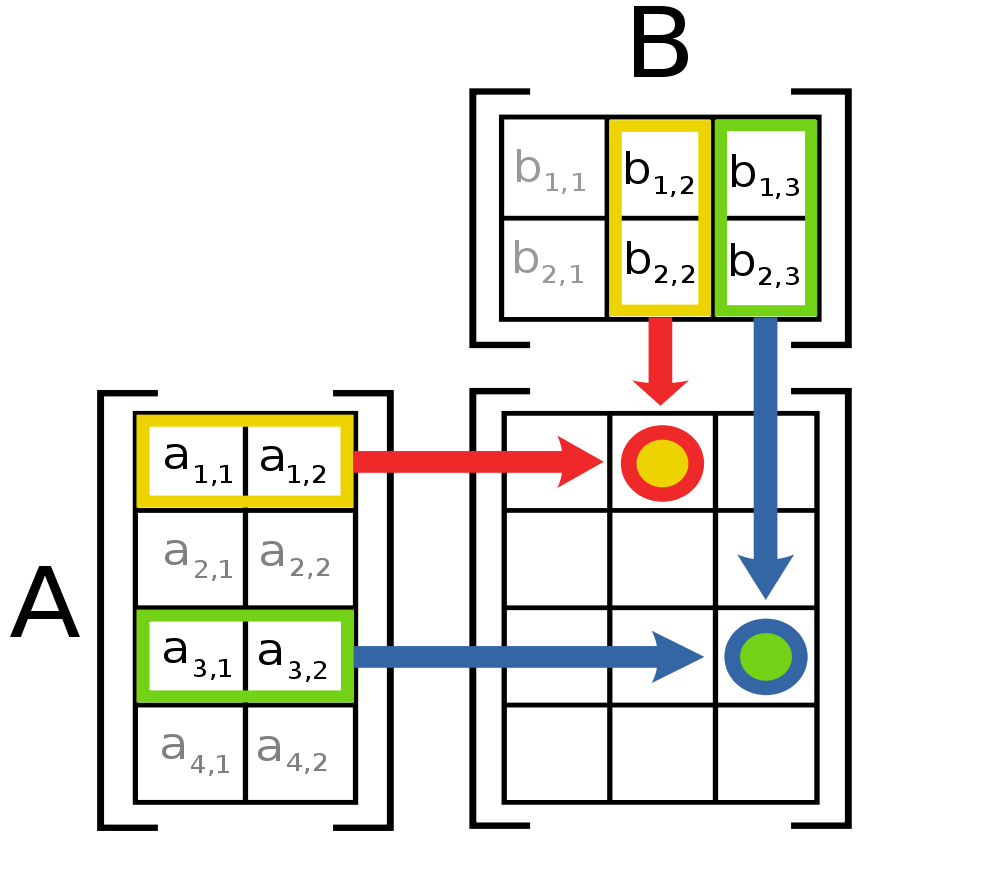
\includegraphics[width=0.5\linewidth]{matrix_mul}
\caption{Principle of the matrix multiplication \cite{wiki_matrix_mul}.}
\label{fig:matrix_mul}
\end{figure}

This chapter will take a look at different implementations of the matrix multiplication for both, the CPU and the GPU. For simplicity, square matrices are used and stored as one dimensional arrays in row major order.

\subsection{CPU Implementation}
\label{sec:matrix_cpu_implementation}

Although several optimized implementations exist we will first have a detailed look at a simple naive implementation as given in listing \ref{lst:matrix_cpu}.

\lstset{basicstyle=\ttfamily{}\scriptsize{}}
\lstinputlisting[language=C++, caption=A simple C++ implementation of a square matrix multiplication for the CPU., label=lst:matrix_cpu, firstline=15, lastline=26]{code/matrix/main.cpp}
\lstset{basicstyle=\ttfamily{}}

The \lstinline!matrixMul()! function takes two pointers to the memory where the two input matrices are stored, another pointer to already allocated memory where the output is written to and a final \lstinline!size! parameter giving the edge length of the input and output matrices.
The algorithm itself is simple. Every element of the output matrix has to be calculated, therefore the outer two \lstinline!for! loops run through all of these elements. For each output element the dot product of the \lstinline!row! in matrix \lstinline!a! and the \lstinline!col! in matrix \lstinline!b! are calculated.

The performance of this implementation is conceivably slow as one can see in figure \ref{fig:matrix_chart}. Multiplying matrices with an edge length of up to 700 elements can be done in a short time (below one second), but larger matrices require a huge period of time which is unsatisfying in most cases.

\subsection{Naive GPU implementation}

A working GPU implementation can be directly derived from the simple CPU implementation given in the previous chapter \ref{sec:matrix_cpu_implementation}. As we can see in figure \ref{fig:matrix_mul}, each output element is calculated independently and the calculation of an output element corresponds to the loop body of the second \lstinline!for! loop in the CPU implementation in listing \ref{lst:matrix_cpu}. Therefore, both outer \lstinline!for! loops offering a good starting point for parallelization. 

The naive GPU implementation seen in listing \ref{lst:matrix_cl_naive} uses the same principle as the initial CPU version. To simplify the code listing context and command queue have already been created and are provided as input to the \lstinline!matrixMulCL()! function.
For the three buffers holding the two input matrices and the output matrix OpenCL buffers have to be created. On creation, additional flags may be provided to allow the underlying OpenCL implementation to optimize memory access to these buffers. Therefore, the two input matrix buffers are set to \lstinline!CL_MEM_READ_ONLY! and the output buffer is set to \lstinline!CL_MEM_WRITE_ONLY!. These flags only affect access to the memory object from the kernel code and do not restrict the host application to read or write buffers. 
After the buffers have been created, a write operation is enqueued on the command queue to the GPU for both input matrices. Note, that the third parameter of the calls to \lstinline!clEnqueueWriteBuffer()! specifies whether the function blocks until the write operation has completed or not. This parameter is set to \lstinline!false! allowing OpenCL to transfer the memory blocks asynchronously to the running host application and even in parallel .
Before the kernel can be executed, the two input buffers, the output buffer and the size of the matrix are set as arguments to the \lstinline!__kernel! function. Furthermore the global and local work size for the kernel execution have to be determined. The global work size must be a multiple of the used work group size (local work size). The chosen size of the work groups affects GPU utilization as a too small size may lead to wasted processing powers on the SMs and decreases latency tolerance. A too large work group size may cause the kernel to fill up the available register file on the SM in which case local variables are moved to global memory causing a serious drop in performance. Finding the optimal work group size is strongly hardware dependent and often boils down to simple try and error.
Note that choosing a work group size which does not evenly divide the global work size and therefor rounding the global work size to the next multiple of the work group size causes the GPU to execute the kernel for additional unneeded work items. Concerning the matrix multiplication example, the kernel would be executed for a bigger matrix with an edge length evenly dividable by the work group size. This has to be kept in mind when e.g. accessing buffers inside the kernel.

After global and local work size have been chosen, the kernel can be enqueued on the command queue to be executed by calling \lstinline!clEnqueueNDRangeKernel()!. The call immediately returns as the kernel is executed asynchronously when the command queue is flushed (\lstinline!clFlush()!) or a blocking command is enqueued, which is the case on the subsequent read operation. The call to \lstinline!clEnqueueReadBuffer()! reads the result back from the device to the host application's array. Note that the third parameter is set to \lstinline!true! indicating a blocking operation. All previously enqueued commands are ensured to be executed and finished before the read operation takes place which returns after all data has been successfully copied to client memory.

\lstset{basicstyle=\ttfamily{}\scriptsize{}}
\lstinputlisting[language=C++, caption=Host code for a matrix multiplication implementation using OpenCL., label=lst:matrix_cl_naive, firstline=29, lastline=55]{code/matrix/main.cpp}
\lstset{basicstyle=\ttfamily{}}

The last missing component of the naive GPU implementation is the OpenCL kernel itself which is given in listing \ref{lst:matrix_cl_naive_kernel}. The \lstinline!__kernel! function closely resembles the loop body of the second \lstinline!for! loop of the CPU implementation in listing \ref{lst:matrix_cpu}. The purpose of a single invocation of this kernel is to calculate one element of the output matrix. By using OpenCL's built-in function \lstinline!get_global_id()! with the dimension as argument, the kernel invocation can retrieve it's position inside the NDRange which equals the output matrix (plus extra space due to work group size rounding). Therefore, the retrieved position has to be checked against the matrices' size as the NDRange may be larger than the original matrix. If the coordinates identify a valid matrix position, the output element is again determined by calculating the dot product of the \lstinline!row! in matrix \lstinline!a! and the \lstinline!col! in matrix \lstinline!b! and eventually written to the output matrix buffer \lstinline!c!.

\lstset{basicstyle=\ttfamily{}\scriptsize{}}
\lstinputlisting[language=CL, caption=OpenCL Kernel code calculating a single element of the output matrix., label=lst:matrix_cl_naive_kernel]{code/matrix/Mult.cl}
\lstset{basicstyle=\ttfamily{}}

When run on the GPU, the performance of this naive OpenCL implementation is already amazingly fast when we have a look at the benchmark in figure \ref{fig:matrix_chart}. At an edge length of 800 elements, the size where the CPU implementation's needed time started to blow up beyond several seconds, the GPU variant still runs very happily at around 200 milliseconds. Additionally, the curve raises far slower than the CPU's one.


\subsection{Optimized GPU implementation}
options for performance improvement
multiple elements per work item

texture unit

\subsubsection{Using vector instructions}
vector instructions (AMD Tile)


\subsubsection{Using local memory}
caching in local memory (blocks)

\subsection{Existing implementations}

Beside the presented implementations, several libraries exist supporting matrix multiplication.

\begin{description}
   \item[clAmdBlas] \hfill \\
   A BLAS (Basic Linear Algebra Subprograms) library provided by AMD.
   \item[cuBlas] \hfill \\
   A BLAS (Basic Linear Algebra Subprograms) library provided by NVIDIA shipped with the CUDA Computing SDK.
\end{description}

\subsection{Benchmarks and conclusion}
Which implementation is when better?

\begin{figure}
\centering
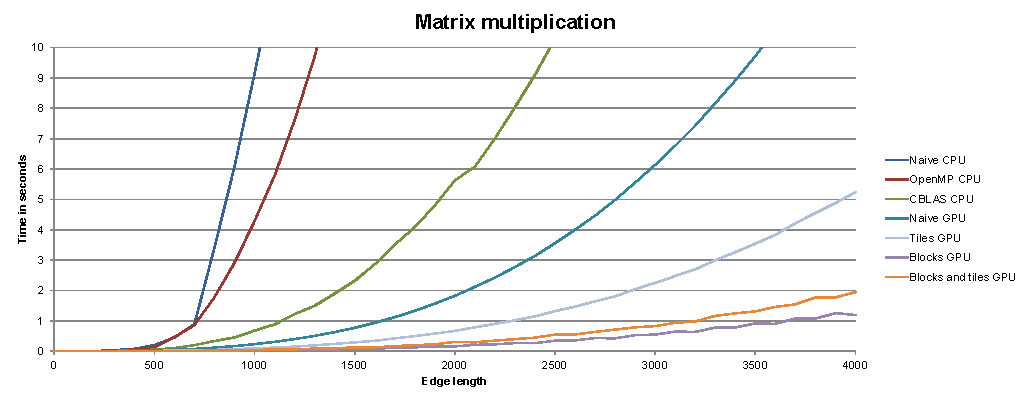
\includegraphics[width=1.0\linewidth]{matrix_chart}
\caption{Benchmark of several square matrix multiplication implementations. CPU implementations are drawn as dashed lines.}
\label{fig:matrix_chart}
\end{figure}

Which problem size?
Which hardware?

